\begin{figure}[t]
\begin{center}
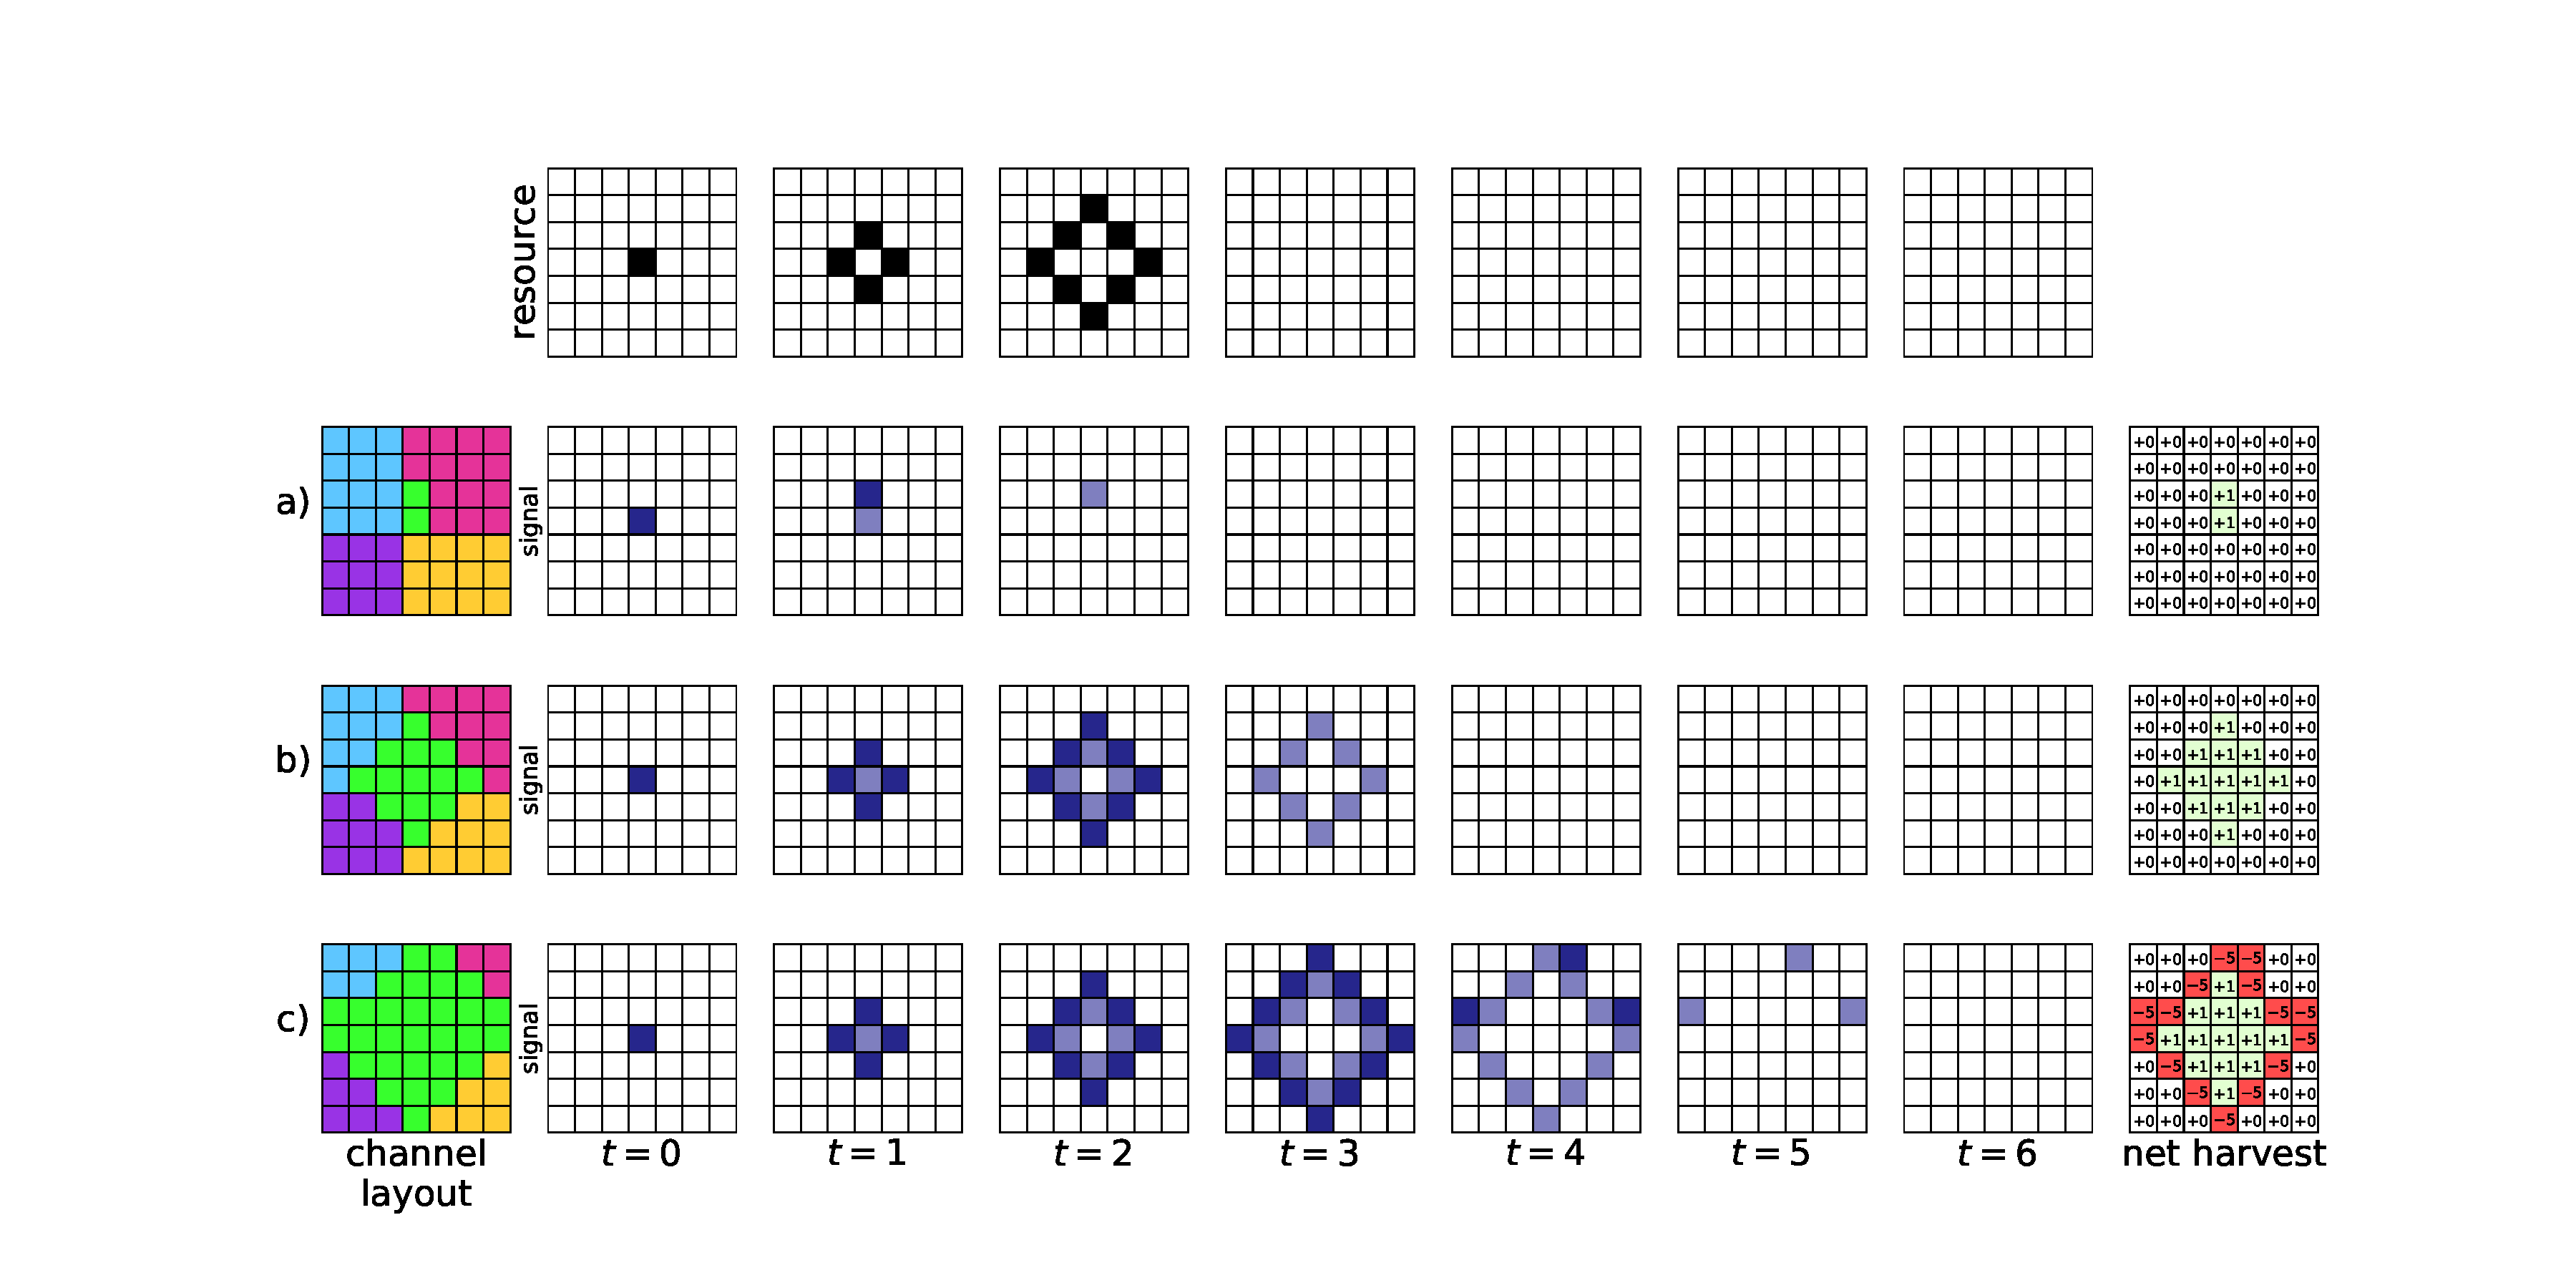
\includegraphics[width=\columnwidth,trim={4cm 0.5cm 4cm 0.5cm},clip]{img/explanatory}
\caption{
\textbf{Activation signaling, and net resource collection for three different-sized same-channel networks during a resource wave event.}
At the top, a resource wave is depicted propagating over three updates and then ceasing for four updates (left to right).
In row $a$, a small two-cell channel-signaling group (far left, in green) is activated; tracking the resource wave (top) yields a small net resource harvest (far right).
In row $b$, an intermediate-sized 13-cell channel-signaling group yields a high net resource harvest.
Finally, in row $c$, a large 29-cell channel-signaling group incurs a net negative resource harvest.
In rows $a$, $b$, and $c$, dark purple indicates the active state, light purple indicates the quiescent state, and white indicates the ready state.
}
\label{fig:explanatory}
\end{center}
\end{figure}
